% Source-faithful schematic draft: 2004 Hunan Arts Q21, PDF p.2 (printed p.177).
% Source ID: src-69c1d502b386b3e69e4b98d9f5500c36d4b278d52aa54448a71182edf7c03358
% Source SHA-256: dc0e39533bc2dd37833ae2dc4bdb93e31a39d08808c842611458bf0b844aaeed
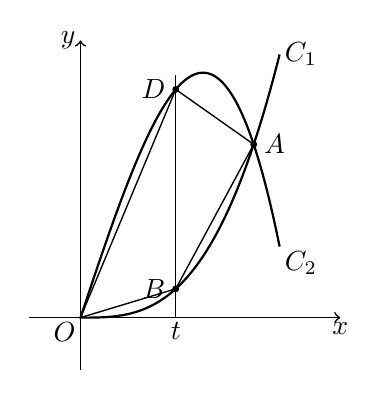
\begin{tikzpicture}[line width=0.6pt,scale=2.2,every node/.style={inner sep=1.5pt}]
  % Axes
  \draw[->] (-0.3,0) -- (1.5,0) node[below] {$x$};
  \draw[->] (0,-0.3) -- (0,1.6) node[left] {$y$};
  \node[below left] at (0,0) {$O$};

  % Curves C1: y = x^3 and C2: y = -2x^3 + 3x
  \draw[thick,domain=0:1.15,samples=60,smooth] plot (\x, {\x*\x*\x}) node[right] {$C_1$};
  \draw[thick,domain=0:1.15,samples=60,smooth] plot (\x, {-2*\x*\x*\x + 3*\x}) node[below right] {$C_2$};

  % Intersection A at (1, 1)
  \coordinate (O) at (0,0);
  \coordinate (A) at (1,1);
  \fill (A) circle (0.02) node[right=2pt] {$A$};

  % Line x = t (choose t = 0.55 for visual fidelity)
  \def\tval{0.55}
  \coordinate (B) at (\tval, {\tval*\tval*\tval});
  \coordinate (D) at (\tval, {-2*\tval*\tval*\tval + 3*\tval});

  % Vertical secant line x = t
  \draw[line width=0.45pt] (\tval, 0) -- (\tval, 1.4);
  \node[below] at (\tval, 0) {$t$};

  % Quadrilateral ABOD: OD, DA, AB, BO
  \draw[line width=0.5pt] (O) -- (D) -- (A) -- (B) -- cycle;

  \fill (B) circle (0.02) node[left=2pt] {$B$};
  \fill (D) circle (0.02) node[left=2pt] {$D$};
\end{tikzpicture}
